\section{Drawing a function}

Lua computes the points needed to draw the curve. Their number is set by the option \tkzname{samples}. \TIKZ\ then draws the line through these points.

\subsection{Defining a function: \tkzcname{tkzFnDef}}

\begin{NewMacroBox}{tkzFnDef}{\marg{name}\marg{expression}}
\emph{Defines a function of the variable \texttt{x}. The name is a Lua name (letters, digits, \texttt{\_}). The function is then referred to by its name in every macro: \tkzcname{tkzFnDraw}\texttt{(f)}, \tkzcname{tkzFnTangent}\texttt{(f,1)}, \tkzcname{tkzFnArea}\texttt{(f)}, etc. In Lua, it is stored in the table \texttt{FN}: \texttt{FN.f(2)}.}

\begin{tabular}{lll}
\toprule
arguments             & example & explanation  \\
\midrule
\TAline{name}{f}{name of the function}
\TAline{expression}{x\string^3-2*x}{Lua expression in x}
\bottomrule
\end{tabular}
\end{NewMacroBox}

\subsection{Drawing a function: \tkzcname{tkzFnDraw}}

\begin{NewMacroBox}{tkzFnDraw}{\oarg{options}\parg{name} \textrm{or} \oarg{options}\marg{expression}}
\emph{The function is given by its name, or directly by its expression; the option \tkzname{name} then gives it a name.}

\begin{tabular}{lll}
\toprule
options             & default & definition     \\
\midrule
\TOline{domain}{xmin:xmax}{domain of the drawing}
\TOline{samples}{200}{number of computed points}
\TOline{name}{}{name given to the function}
\TOline{clip}{true}{the curve is clipped to the window}
\TOline{mark=\dots}{}{a mark at each computed point (\tkzname{plotmarks})}
\TOline{smooth}{}{curve smoothed by \TIKZ}
\bottomrule
\end{tabular}

\emph{Other options are \TIKZ\ options; the style is \tkzname{tkzfn curve}.}
\end{NewMacroBox}

\tkzHand The coordinate system must be initialized with \tkzcname{tkzFnInit} before \tkzcname{tkzFnDraw} is used.

\tkzHand The curve is interrupted where the function is not defined (|ln(x)| for $x\leq 0$) and where it jumps from one side of the window to the other (vertical asymptote).

%<--------------------------------------------------------------------------->
\subsection{Option: \tkzname{samples}}

Two points are enough to draw a line: \tkzname{samples=2}. Here 400 points are requested; the default value is 200.

\begin{tkzexample}[latex=7cm]
\begin{tikzpicture}[scale=1]
    \tkzFnInit[xmin=0,xmax=5,
               ymin=0,ymax=2]
    \tkzFnGrid[sub]
    \tkzFnAxes
    \tkzFnDraw[samples=400,
               domain=.5:5]{1/x}
\end{tikzpicture}
\end{tkzexample}

%<--------------------------------------------------------------------------->
\subsection{Options: \tkzname{xstep, ystep}}

\begin{tkzexample}[]
\begin{tikzpicture}
\tkzFnInit[xmin=0,xmax=110,xstep=10,
           ymin=0,ymax=6,ystep=1]
\tkzFnAxisX[label={\textit{Age}},
            label style={below=12pt,left}]
\tkzFnAxisY[label={\textit{Liters}}]
\tkzFnDraw[domain=0.1:100]{50/x}
\end{tikzpicture}
\end{tkzexample}

\subsection{Changing \tkzname{xstep} and \tkzname{ystep}}

This time the domain goes from 0 to 700 and the values of the function from $0$ to $\tkzFnPrint{1200}$. With \tkzname{tkz-fct}, you had to write |\x| instead of $x$ and |1./90000| instead of |1/90000|; this is no longer necessary.

\begin{tkzexample}[vbox]
\begin{tikzpicture}[scale=1.5]
 \tkzFnInit[xmin=0,xmax=700,xstep=100,
            ymin=0,ymax=1200,ystep=400]
 \tkzFnGrid(0,0)(700,1200)  \tkzFnAxes
 \tkzFnDraw[color=red,samples=100,line width=0.8pt,domain=0:700]
        {(1/90000)*x^3-(1/100)*x^2+(113/36)*x}
\end{tikzpicture}
\end{tkzexample}

\subsection{\tkzname{ystep} and constant functions}

With \tkzname{gnuplot}, |80/6| was an integer division and you had to write |80.|; with Lua, computations are always done with decimal numbers.

\begin{tkzexample}[vbox]
 \begin{tikzpicture}[scale=0.4]
 \tkzFnInit[xmin=0,xmax=30,ymin=0,ymax=90,ystep=6]
 \tkzFnAxisX[ticks=false,label=$t$]
 \tkzFnAxisY[ticks=false,label=$P$]
 \tkzFnDraw[line width=1pt,color=red,dashed,domain=0:30]{80}
 \tkzFnDraw[line width=1pt,color=blue,domain=0:30]{80/(1+4*exp(-0.21*x))}
 \tkzFnText[above,color=red](20,80){$P=80$}
\end{tikzpicture}
\end{tkzexample}

\subsection{Linear functions}
Two points are enough to draw a line: \tkzname{samples=2}.

\begin{tkzexample}[vbox]
 \begin{tikzpicture}[]
 \tkzFnInit[xmin=0,xmax=10,ymin=0,ymax=20,ystep=5]
 \tkzFnAxes
 \tkzFnDraw[color=red,domain=0:10,samples=2]{2*x+5}
 \tkzFnDraw[color=blue,domain=0:10,samples=2]{-x+15}
 \tkzFnDraw[color=green,domain=0:10,samples=2]{7}
\end{tikzpicture}
\end{tkzexample}

%<--------------------------------------------------------------------------->
\subsection{Subgrid}

   $y=(x-4)\text{e}^{-0.25x+5}$

Another grid can be drawn on a part of the window.

\begin{tkzexample}[latex=8cm]
\begin{tikzpicture}[scale=.8]
 \tkzFnInit[xmin=4,xmax=18,xstep=2,
            ymin=20,ymax=90,ystep=10]
 \tkzFnDraw[domain=5:18]
        {(x-4)*exp(-0.25*x+5)}
 \tkzFnGrid(4,20)(18,90)
 \tkzFnAxes
 \tkzFnGrid[sub,
            subdx=0.5,
            subdy=2,
            color=brown](6,60)(12,90)
\end{tikzpicture}
\end{tkzexample}

%<--------------------------------------------------------------------------->
\subsection{Text and points}

\begin{center}
\begin{tkzexample}[vbox]
\begin{tikzpicture}[scale=2]
 \tkzFnInit[xmin=-3,xmax=3,ymin=-1,ymax=4]
 \tkzFnGrid[sub,subdx=.5,subdy=.5]
 \tkzFnAxes
 \tkzFnDraw[domain=-3:2]{(2-x)*exp(x)}
 \tkzFnText(-2,1.25){$\mathcal{C}_{f}$}
 \tkzFnDefPointXY[draw](2,0){A}
 \tkzFnLabelPoints(A)
\end{tikzpicture}
\end{tkzexample}
\end{center}

\endinput
